\begin{maintask}{1-B}
  \subsection*{課題内容}
  IPv4ではARP，IPv6では近隣探索で相手のMACアドレスを調べ，そのパケットのやり取りを確認した.

  \subsection*{実験方法}
  \begin{enumerate}
    \item 実行前の近隣キャッシュを記録
      \begin{minted}{zsh}
        ip ne
      \end{minted}

    \item 1つ目のターミナルでキャプチャを開始
      \begin{minted}{zsh}
        tcpdump -i eth1 -s 0 -w B.pcap 'not port 4200'
      \end{minted}

    \item キャプチャ中に，別のターミナルでarping，ndisc6を実行
      \begin{minted}{zsh}
        (IPv4) arping -c 3 172.28.0.200
        (IPv6) ndisc6 2001:2f8:40:11da::200 eth1
      \end{minted}

    \item 実行後に近隣キャッシュを再度記録
      \begin{minted}{zsh}
        ip ne
      \end{minted}

    \item キャプチャ側でCtrl-Cを押し，pcapをダウンロードしてWiresharkで開く
  \end{enumerate}

  \subsection*{結果}
  tcpdumpの実行結果，実行前後の近隣キャッシュ，arpingとndisc6の実行結果をそれぞれ
  出力\ref{out:tcpdump_b}，
  出力\ref{out:ne_before}，
  出力\ref{out:arping}，
  出力\ref{out:ndisc6}，
  出力\ref{out:ne_after}
  に示した．

  \begin{termout}[H]
    \caption{tcpdump の実行結果}\label{out:tcpdump_b}
    \begin{minted}{zsh}
    guest@host82:~$ tcpdump -i eth1 -s 0 -w B.pcap 'not port 4200'
    tcpdump: listening on eth1, link-type EN10MB (Ethernet), capture size 262144 bytes
    ^C498 packets captured
    500 packets received by filter
    0 packets dropped by kernel
    \end{minted}
  \end{termout}

  \begin{termout}[H]
    \caption{実行前の近隣キャッシュ}\label{out:ne_before}
    \begin{minted}{zsh}
    guest@host82:~$ ip ne
    172.28.0.203 dev eth1 lladdr e6:aa:7d:51:5c:ed STALE
    172.28.0.200 dev eth1 lladdr fe:89:01:c2:83:3a STALE
    172.28.0.1 dev eth1 lladdr a2:1e:33:b9:98:ef REACHABLE
    fe80::e4aa:7dff:fe51:5ced dev eth1 lladdr e6:aa:7d:51:5c:ed REACHABLE
    fe80::a01e:33ff:feb9:98ef dev eth1 lladdr a2:1e:33:b9:98:ef router REACHABLE
    2001:2f8:40:11da::1 dev eth1 lladdr a2:1e:33:b9:98:ef router REACHABLE
    \end{minted}
  \end{termout}

  \begin{termout}[H]
    \caption{arping(IPv4) の実行結果}\label{out:arping}
    \begin{minted}{zsh}
    guest@host82:~$ arping -c 3 172.28.0.200
    ARPING 172.28.0.200 送信元 172.28.0.182 eth1
    ユニキャスト 応答 送信元 172.28.0.200 [FE:89:01:C2:83:3A]  0.742ミリ秒
    ユニキャスト 応答 送信元 172.28.0.200 [FE:89:01:C2:83:3A]  0.522ミリ秒
    ユニキャスト 応答 送信元 172.28.0.200 [FE:89:01:C2:83:3A]  0.520ミリ秒
    3 プローブを送信 (1 ブロードキャスト)
    3 応答を受信
    \end{minted}
  \end{termout}

  \begin{termout}[H]
    \caption{ndisc6(IPv6) の実行結果}\label{out:ndisc6}
    \begin{minted}{zsh}
    guest@host82:~$ ndisc6 2001:2f8:40:11da::200 eth1
    Soliciting 2001:2f8:40:11da::200 (2001:2f8:40:11da::200) on eth1...
    Target link-layer address: FE:89:01:C2:83:3A
    from 2001:2f8:40:11da::200
    \end{minted}
  \end{termout}

  \begin{termout}[H]
    \caption{実行後の近隣キャッシュ}\label{out:ne_after}
    \begin{minted}{zsh}
    guest@host82:~$ ip ne
    172.28.0.203 dev eth1 lladdr e6:aa:7d:51:5c:ed STALE
    172.28.0.200 dev eth1 lladdr fe:89:01:c2:83:3a STALE
    172.28.0.1 dev eth1 lladdr a2:1e:33:b9:98:ef REACHABLE
    fe80::fc89:1ff:fec2:833a dev eth1 lladdr fe:89:01:c2:83:3a REACHABLE
    fe80::e4aa:7dff:fe51:5ced dev eth1 lladdr e6:aa:7d:51:5c:ed STALE
    fe80::a01e:33ff:feb9:98ef dev eth1 lladdr a2:1e:33:b9:98:ef router REACHABLE
    2001:2f8:40:11da::1 dev eth1 lladdr a2:1e:33:b9:98:ef router DELAY
    \end{minted}
  \end{termout}

  \begin{figure}[htbp]
    \centering
    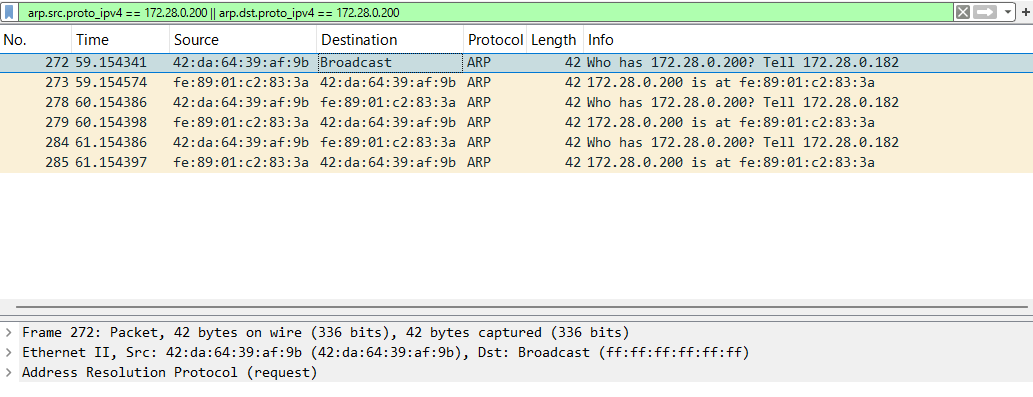
\includegraphics[width=0.98\columnwidth]{fig/wireshark_arp.png}
    \caption{ARPのやり取りをWiresharkで読み取った結果}
    \label{fig:ws_arp}
  \end{figure}

  \begin{figure}[htbp]
    \centering
    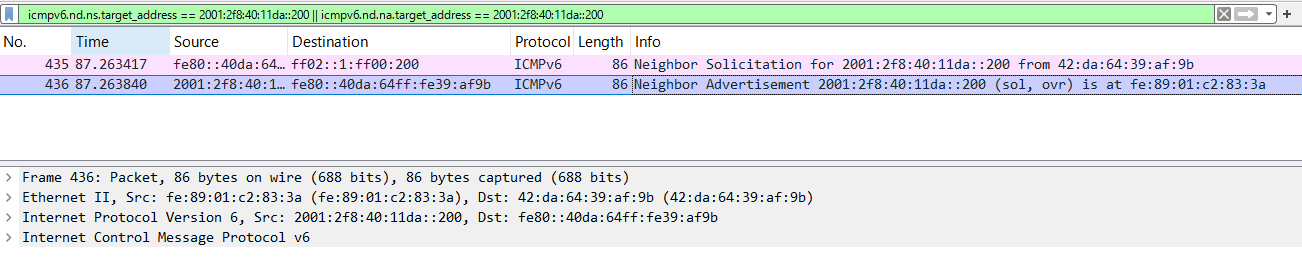
\includegraphics[width=0.98\columnwidth]{fig/wireshark_nd.png}
    \caption{NDのやり取りをWiresharkで読み取った結果}
    \label{fig:ws_nd}
  \end{figure}

  IPv4では，arpingにより172.28.0.200のMACアドレスが\texttt{FE:89:01:C2:83:3A}であると分かった．出力\ref{out:arping}には「3プローブを送信(1ブロードキャスト)」とあり，最初の1回がブロードキャストのARP Requestで，残りの2回はMACアドレスが分かった後のユニキャストであると読み取れる．図\ref{fig:ws_arp}では，No.272のARP Requestの宛先がBroadcast(ff:ff:ff:ff:ff:ff)で，``Who has 172.28.0.200? Tell 172.28.0.182''という内容になっており，No.273のARP Replyでは172.28.0.200が\texttt{fe:89:01:c2:83:3a}にいると返答している．続くNo.278とNo.284のRequestは宛先が\texttt{fe:89:01:c2:83:3a}のユニキャストで，それぞれNo.279，No.285でReplyが返っている．これは出力\ref{out:arping}の「1ブロードキャスト」の内訳と一致する．

  IPv6では，ndisc6により2001:2f8:40:11da::200のMACアドレスが，IPv4と同じ\texttt{FE:89:01:C2:83:3A}であると分かった．これはIPv4とIPv6の双方で，同一のホスト(sshd)のMACアドレスが得られたことを示す．図\ref{fig:ws_nd}では，No.435のNeighbor Solicitation(Type 135)が，宛先\texttt{ff02::1:ff00:200}（2001:2f8:40:11da::200に対するsolicited-nodeマルチキャストアドレス）に送られている．その直後のNo.436のNeighbor Advertisement(Type 136)は，2001:2f8:40:11da::200から要求元へユニキャストで返され，Target link-layer addressとして\texttt{fe:89:01:c2:83:3a}が通知されている．ARPがブロードキャストを使うのに対し，NDでは対象のアドレスに対応するマルチキャストグループ宛てにSolicitationを送る点が異なる．

  近隣キャッシュは，出力\ref{out:ne_before}と出力\ref{out:ne_after}を比べると，\texttt{fe80::fc89:1ff:fec2:833a}のエントリが新たに追加され，そのMACアドレスは上記と同じ\texttt{fe:89:01:c2:83:3a}であった．このアドレスは，MACアドレスからEUI-64形式で作られたリンクローカルアドレスである．一方，172.28.0.200のエントリは実行前から存在し(STALE)，実行後も変化していなかった．それにもかかわらず，arpingはNo.272でブロードキャストのRequestを送信している．
\end{maintask}
